% Этот шаблон документа разработан в 2014 году
% Данилом Фёдоровых (danil@fedorovykh.ru) 
% для использования в курсе 
% <<Документы и презентации в \LaTeX>>, записанном НИУ ВШЭ
% для Coursera.org: http://coursera.org/course/latex .
% Вы можете изменять, использовать, распространять
% этот документ любым способом по своему усмотрению. 
% В качестве благодарности автору вы можете сохранить 
% в начале документа данный текст или просто ссылку на
% http://coursera.org/course/latex
% Исходная версия Шаблона --- 
% https://www.writelatex.com/coursera/latex/1.1


\documentclass[a4paper,12pt]{article}

\usepackage{cmap}					% поиск в PDF
\usepackage[T2A]{fontenc}			% кодировка
\usepackage[utf8]{inputenc}			% кодировка исходного текста
\usepackage[english,russian]{babel}	% локализация и переносы
\usepackage{amsfonts}
\usepackage{amsmath}
\usepackage{hyperref}
\usepackage{amsthm}
\usepackage{empheq}
\usepackage[most]{tcolorbox}
\usepackage{graphicx}
\graphicspath{{./}}

\newtcbox{\bluebox}[1][]{%
    nobeforeafter, math upper, tcbox raise base,
    enhanced, colframe=blue!30!black,
    colback=blue!30, boxrule=1pt,
    #1}

\newcommand{\expec}{\mathbb{E}}
\newcommand{\disp}{\mathbb{D}}
\newcommand{\orst}[2]{#1_{(#2)}}
\newcommand{\normal}[2]{\mathcal{N}(#1,\,#2)}
\newcommand{\indep}{\perp \!\!\! \perp}
\newcommand{\pconv}{\overset{P}{\to}} 
\newcommand{\sconv}{\overset{a. e.}{\to}}
\newcommand{\sconvt}{\overset{P_\theta \,\,a. e.}{\to}}
\newcommand{\dconv}{\overset{d}{\to}}
\newcommand{\dconvt}{\overset{d_{\theta}}{\to}}
\newcommand{\grad}{\nabla}
\newcommand{\sumin}{\sum\limits_{i=1}^n}
\newcommand{\prodin}{\prod\limits_{i=1}^n}
\newcommand{\sample}{X_1, X_2, ..., X_n}
\newcommand{\derb}[1]{\frac{\partial}{\partial #1}}
\newcommand{\gendis}{P \in \{ P_\theta : \theta \in \Theta \subset \R^d\}}

\newcommand{\R}{\mathbb{R}}
\DeclareMathOperator*\lowlim{\underline{lim}}
\DeclareMathOperator*\uplim{\overline{lim}}
\DeclareMathOperator*{\argmin}{argmin}
\DeclareMathOperator*{\argmax}{argmax}

\renewcommand*{\proofname}{Доказательство}
\newcommand{\task}[1]{\noindent\textbf{Задача #1}\\}
\newcommand{\sol}{\noindent\textbf{Решение: }}

\newenvironment{annotation}{\begin{center}
    \begin{tabular}{|p{0.9\textwidth}|}
    \hline\\
}
{ 
    \\\\\hline
    \end{tabular} 
    \end{center}
}
\newtheorem{dfn}{Определение}[section]
\newtheoremstyle{named}{}{}{\itshape}{}{\bfseries}{}{.5em}{#1\,\thmnote{(#3)}}
\theoremstyle{named}
\newtheorem*{namedtheorem}{Теорема}

\newtheorem{claim}{Утверждение}

\author{Паненко Семён по конспектам Троешестовой Лидии}
\title{Математическая статистика, конспекты}
\date{\today}

\begin{document} % Конец преамбулы, начало текста.
\maketitle
\tableofcontents
\section{Основы математической статистики}
Предмет математической статистики: из экспериментальных данных понять природу явления.
Пусть заданы следующие величины:
\begin{itemize}
    \item $X_1, ..., X_n$ - некоторые числовые характеристики многократного эксперимента
    \item $\mathcal{X} $ - выборочное пространство, множество всевозможных значений чиселнны характеристик
    \item $\mathcal{B(X)}$ - $\sigma$-алгебра на $X$, нужна, чтобы ввести распределения на $X$
\end{itemize}
\begin{dfn}
    Вероятностно-статистической моделью называется тройка $(\mathcal{X}, \mathcal{B(X)}, \mathcal{P})$, удовлетворяющая 
    написанным выше условиям
\end{dfn}
Вероятностно-статистическая модель нужна, чтобы математически моделировать случайный эксперимент. Если нам нужна выборка размера 
$n$, то можно взять ВСМ $(\mathcal{X}^n, \mathcal{B}(X^n), \mathcal{P})$. Если нужно промоделировать бесконечную выборку, 
то стоит взять $(\mathcal{X}^\infty, \mathcal{B(X^\infty)}, \mathcal{P})$, в которой сигма-алгебра порождена всевозможными конечными 
произведениями борелевский множеств в каждом из сомножителей декартового произведения. 
\begin{dfn}
    Выборкой называется вектор независимых, одинаково распределённых случайных величин.
\end{dfn}
\subsection{Методы вывода}
Существует два основных метода вывода:
\begin{enumerate}
    \item Параметрический: неизвестное распределение может быть параметризовано некоторым параметром $\theta \in \Theta$, то есть 
    $$
        \mathcal{P} = \{P_\theta : \theta \in \Theta\}
    $$
    Наша задача в этом случае заключается в том, чтобы определить как можно 
    более точно значение параметра $\theta$
    \item Непараметрический: неизвестные распределения не могут быть или не параметризуются естественным образом. Наша цель в таком 
    случае определить функцию распределения или плотность неизвестного неизвестного распределения.
\end{enumerate}
Также существуют два возможных способа вывода:
\begin{enumerate}
    \item Частотный: Построение суждений о неизвестном распределении $P$ строятся на предеположении, что все распределения из 
    $\mathcal{P}$ равноправны. 
    \item Байесовский: Мы считаем, что на множестве всех распределений задано некоторое распределение, которое мы называем 
    "априорным знанием" 
\end{enumerate}
\subsection{Методы численного вычисления интегралов}
\subsubsection{Метод прямоугольников}
Мы хотим вычислить $I = \int_{a}^b f(x) dx$. Разобъём интервал интегрирования:
$$
    a = x_0 < x_1 < ... < x_n = b
$$
Тогда в качестве оценки интеграла рассмотрим величину:
$$
    \hat I = \sumin f\left(\frac{x_{i-1} + x_i}{2}\right)(x_i - x_{i-1})
$$
Например, в качестве разбиения можно рассмотреть равномерную сетку:
$$
    x_i = x_0 + id, \quad d = \frac{b-a}{n}
$$
Тогда оценка интеграла запишется в виде:
$$
    \hat I = \sumin \left(\frac{b-a}{n}\right)f\left(a + \left(\frac{i-1}{2}\right)\frac{b-a}{n}\right)
$$
\begin{namedtheorem}
    Пусть $f$ - дважды непрерывно дифференцируемая функция. Тогда при испльзовании равномерной сетки выполнена оценка:
    $$
        |\hat I - I| \leq \frac{M(b-a)^3}{24n^2}, \quad M = \max_{x\in [a, b]}|f^{\prime\prime}(x)|
    $$
\end{namedtheorem}
Доказательство: Разложим $f(x)$ по формуле Тейлора с остаточным членом:
$$
    f(x) = f(r_i) + f^\prime(x - r_i) + \frac{1}{2}f^{\prime\prime}(z(x))(x-r_i)^2
$$
Где $r_i = \frac12(x_{i-1} + x_i)$. Заметим, что по формуле интегрирования по частям, выполнено равенство:
$$
    \int_{x_{i-1}}^{x_i} f^\sample(r_i)(x - r_i)dx = 0
$$
Тогда:
$$
    R_i = \int_{x_{i-1}}^{x_i} f(x) - f(r_i) dx = \frac{1}{2}\int_{x_{i-1}}^{x_i} f^{\prime\prime}(z(x))(x-r_i)^2 dx
$$
Тогда из предположений теоремы:
$$
    |R_i| \leq \frac{M}{2}\frac{(x-r_i)^3}{3} \leq \frac{M(b-a)^3}{24n^2}
$$
Таким образом, для достаточно "хороших" функций погрешность метода имеет асимптотику $\frac{1}{n^2}$
\subsubsection{Метод Монте-Карло}
Пытаемся вычислить интеграл $I = \int_{a}^b f(x) dx$. Рассмотрим также случайную величину $\xi \sim U[a, b]$. 
Заметим, что:
$$
    I = \int_{a}^b f(x) dx = (b-a)\left[\frac{1}{b-a}\int_{a}^b f(x) dx\right] = \frac{1}{b-a}\expec f(\xi)
$$
Рассмотрим выборку $x_1, ..., x_n$ из распределения $U[0, 1]$. В качестве оценки интеграла выберем:
$$
    \hat I = (b-a)\overline{f(X)}
$$
По УЗБЧ эта оценка почти-наверное сходится к истинному значению интеграла. В предположении конечного $\expec(f(\xi))^2$, то 
по ЦПТ:
$$
    \sqrt{n}\frac{I - \hat I}{(b-a)\sqrt{\disp f(\xi)}} \dconv \eta \sim \normal{0}{1}
$$
По свойствам нормального распределения $P(|\eta| \leq 3) \approx 0$. Поэтому при большиъ $n$ оценка имеет порядок малости $\frac{1}{\sqrt{n}}$
с большой вероятностью 
\subsubsection{Сравнение методов}
\begin{enumerate}
    \item Погрешности: Метод прямоугольников - $\frac{1}{n^2}$, метод Монте-Карло - $\frac{1}{\sqrt{n}}$
    \item Ошибка метода Монте-Карло вероятностная, зависит от $\disp f(\xi)$. 
    \item Для интегралов малой кратности лучше метод прямоугольников 
    \item Для интегралов большой кратности необходимо слишком много точек для сходимости метода, поэтому лучше использовать метод Монте-Карло 
\end{enumerate}

\section{Точечные и интервальные оценки}
Пусть задана вероятностно статистическая модель $(\mathcal{X}^n, \mathcal{B}(X^n), \mathcal{P})$, причём $\mathcal{P} = \{ P_\theta
: \theta \in \Theta\}$, то есть мы имеем дело с параметрическим подходом. Пусть также $X =(\sample)$ - выборка из 
неизвестного распределения этого класса. 
\begin{dfn}
    Пусть $(E, \rho)$ - измеримое пространство. Измеримое отображение $S: \mathcal{X} \to E$ называется статистикой. В случае 
    $E = \Theta$ оно также называется оценкой.
\end{dfn}
\begin{annotation}
    Оценивать можно не только сам параметр, но и измеримые функции от него: $\tau(\theta)$
\end{annotation}
\subsection*{Примеры статистик}
\begin{enumerate}
    \item $\overline{X}, \overline{X^2}, \overline{X^k} = \frac{1}{n}\sumin X_i^k$ - выборочный $k$-ый момент
    \item $S^2 = \overline{X^2} - \overline{X}^2 = \frac{1}{n}\sumin (X_i - \overline{X})^2$ - выборочная дисперсия
    \item Вариационный ряд: $(\orst{X}{1}, \orst{X}{2}, \orst{X}{3}, ...\orst{X}{n})$ - упорядоченная по неубыванию выборка. 
    \item $\orst{X}{k} - k$-ая порядковая статистика 
\end{enumerate}
\subsection{Свойства оценок}
Пусть $X = (\sample)$ - выборка из неизвестного распределения $\gendis$. 

\begin{annotation}
Обозначим через $\expec{}_\theta, \disp{}_\theta, \dconvt, P_\theta$
 - п.н - соответственно математиматическо ожидание, дисперсия, сходимость по распределению для распределения $P_\theta$
\end{annotation}

\begin{dfn}
    Оценка $\hat\theta$ называется несмещённой оценкой параметра $\tau(\theta)$, если выполнено:
    $$
        \forall \theta \in \Theta: \quad \expec_\theta \hat\theta(\sample) = \tau(\theta)
    $$
\end{dfn}
Смысл этого определения заключается в том, что при многократном повторении эксперимента в среднем мы будем получать истинное значение 
параметра.


Примеры:
\begin{enumerate}
    \item $\hat\theta_1 = \overline{X}$, $\hat\theta_1 = X_1$ - несмещённые оценки для $\tau(\theta) = \expec_\theta(X_1)$
    \item $\mathcal{P} = \{ Bern(\theta), \theta \in [0, 1] \}$. Тогда $\overline{X}, X_1$ - несмещённые оценки параметра $\theta$.
    \item $\mathcal{P} = \{ Exp(\theta), \theta > 0 \}$. Тогда $\overline{X}$ - несмещённая оценка параметра $\frac{1}{\theta}$
    \item Рассмотрим оценку $S^2 = \overline{X^2} - \overline{X}^2$. Посчитаем её математиматическое ожидание:
    \begin{equation}
        \begin{split}
        \expec_\theta S^2 &= \expec_\theta\left(\frac{1}{n}\sumin X_i^2\right) - \expec_\theta\left(\frac{1}{n}\sumin X_i\right)^2 \\ 
        &=\expec_\theta X_1^2 - \frac{1}{n^2}\left(n\expec_\theta X_1^2 - (n^2 - n)\expec_\theta(X_1X_2)\right)  \\
        &=\expec_\theta X_1^2 - \frac{1}{n}\expec_\theta X_1^2 - \left(1 - \frac{1}{n}\right)(\expec_\theta X_1) ^2 \\
        &= \frac{n-1}{n}\left(\expec_\theta X_1^2 - \left(\expec_\theta X_1\right)^2 \right)\\
        &= \frac{n-1}{n}\disp_\theta X_1    
        \end{split}
    \end{equation}
    Таким образом, $S^2$ - смещённая оценка дисперсии, а $\frac{n}{n-1}S^2$ - несмещённая.
\end{enumerate}
\subsection*{асимптотические свойства}
Пусть $X = (\sample)$ - выборка из неизвестного распределения $\gendis$. 
\begin{dfn}
    Оценка (последовательность оценок) $\hat\theta$ называется состоятельной оценкой параметра $\tau(\theta)$, если выполнено:
    $$
    \forall \theta \in \Theta: \quad \hat\theta(\sample) \pconv \tau(\theta)
    $$
\end{dfn}
\begin{dfn}
    Оценка (последовательность оценок) $\hat\theta$ называется сильно состоятельной оценкой параметра $\tau(\theta)$, если выполнено:
    $$
    \forall \theta \in \Theta: \quad \hat\theta(\sample) \sconvt \tau(\theta)
    $$
\end{dfn}
\begin{dfn}
    Оценка (последовательность оценок) $\hat\theta$ называется асимптотически нормальной оценкой параметра $\tau(\theta)$, если выполнено:
    $$
    \forall \theta \in \Theta: \quad \sqrt{n}(\hat\theta(\sample) - \theta) \dconv \normal{0}{\Sigma(\theta)}
    $$
    При этом матрица $\Sigma(\theta)$ называется асимптотической матрицей ковариаций. В случае $d = 1$ это число, которое иногда называют 
    асимптотической дисперсией оценки 
\end{dfn}
Смысл:
\begin{enumerate}
    \item Состоятельность - с ростом количества наблюдений вероятность большого отклонения оценки от истинного значения параметра мала.
    \item асимптотическая нормальность - даёт численную характеристику степени отклонения оценки от истинного значения параметра
    \item Сильная состоятельность имеет смысл для данных потсупающих последовательно. С вероятностью 1, пока поступает всё больше и больше 
    объектов выборки, мы приближаемся к истинному значению параметра.
\end{enumerate}
Пример: Пусть $\sample$ - выборка из распределения Лапласа со сдвигом $\theta$. Его плотность:
$$
    p_\theta(x) = \frac{1}{2}e^{-|x-\theta|}
$$
\begin{enumerate}
    \item Согласно закону больших чисел, $\overline{X}$ - сильно состоятельная оценка $\expec_\theta X_1 = \theta$
    \item Согласно центральной предельной теореме, $\overline{X}$ - а.н.о параметра $\theta$ с асмпт. дисперсией $\sigma^2 = 
    \disp_\theta X_1 = 2$ 
\end{enumerate}
\begin{annotation}
    Из сильной состоятельности или асимптотической нормальности следует обычная состоятельность. Другие следствия в общем случае неверны. 
\end{annotation}
\subsection{Наследование свойств оценок}
Пусть есть оценка параметра $\psi(\theta)$ с какими-то свойствами. Наша цель: получить оценку параметра $\varphi(\psi(\theta))$
с такими же свойствами. 
\begin{namedtheorem}[О наследовании сходимостей]
    Пусть $\xi_n \sconv \xi$ - случайные вектора из $\R^m$. Пусть также $h: \, \R^m \to \R^k$ - непрерывная почти всюду 
    относительно распределения $\xi$ функция. Тогда $h(\xi_n) \sconv h(\xi)$
\end{namedtheorem}
\begin{namedtheorem}[О наследовании сходимостей]
    Пусть $\xi_n \pconv \xi$ - случайные вектора из $\R^m$. Пусть также $h: \, \R^m \to \R^k$ - непрерывная почти всюду 
    относительно распределения $\xi$ функция. Тогда $h(\xi_n) \pconv h(\xi)$
\end{namedtheorem}
\begin{namedtheorem}[О наследовании сходимостей]
    Пусть $\xi_n \dconv \xi$ - случайные вектора из $\R^m$. Пусть также $h: \, \R^m \to \R^k$ - непрерывная \textbf{всюду} 
    относительно распределения $\xi$ функция. Тогда $h(\xi_n) \dconv h(\xi)$
\end{namedtheorem}
Пример: Пусть $\xi_n$ - н.о.р.с.в, причём $\expec \xi_n = a\neq 0$. Тогда по УЗБЧ:
$$
    \frac{\sumin X_i}{n} \sconv a = \xi
$$
Применяя теорему о наследовании сходимостей (первый вариант) к последовательности $\xi_n = \frac{S_n}{n}$, и функции $h(x) = \frac{1}{x}$,
получаем, что:
$$
    \frac{n}{\sumin X_i} \sconv h(a) = \frac{1}{a}
$$
\begin{namedtheorem}[Следствие из теоремы о наследовании сходимостей]
    Пусть $\hat\theta$ - (сильно) состоятельная оценка параметра $\tau(\theta)$. Пусть также $f$ непрерывна на $\Theta$. 
    Тогда $f(\hat\theta)$ - (сильно) состоятельная оценка параметра $f(\tau(\theta))$.
\end{namedtheorem}
\begin{namedtheorem}[Лемма Слуцкого]
    Пусть $\{\xi_n\}, \{\eta_n\}$ - последовательности н.о.р.с.в., причём $\xi_n \dconv \xi, \eta_n\dconv c = const$. Тогда выполнено:
    \begin{enumerate}
        \item $\xi_n + \eta_n \to \xi + c$
        \item $\xi_n \times \eta_n \to c\xi$
    \end{enumerate}
\end{namedtheorem}
\begin{annotation}
    Лемма Слуцкого не следует из теоремы о наследовании сходимостей, так как из сходимости по распределению 
    компонент вектора не следует сходимость самого вектора по распределению. 
\end{annotation}
\begin{namedtheorem}[О производной]
    Пусть выполнены следующие условия:
    \begin{enumerate}
        \item $\{\xi_n\}$ - случайные векторы из $\R^d$
        \item $\xi_n \dconv \xi$ 
        \item $h(x): \,\, \R^d \to \R^k$ - непрерывно дифференцируемая в точке $a$ функция 
        \item $b_n \to 0$ - числовая последовательность\\
    \end{enumerate}
    Тогда выполнена следующая сходимость:
    $$
        \frac{h(a + \xi_n b_n) - h(a)}{b_n} \dconv h^\prime(a) \xi
    $$
\end{namedtheorem}
Пример: Пусть $\xi_n$ - н.о.р.с.в., причём $\expec \xi_n = a, \disp \xi_n = \sigma^2$. Тогда по ЦПТ:
$$
    \sqrt{n}\left(\frac{S_n}{n} - a\right) \dconv \normal{a}{\sigma^2}
$$
Применим теорему о производной к последовательности $\xi_n = \sqrt{n}\left(\frac{S_n}{n} - a\right)$, функции $h(x) = \frac{1}{x}$ и числовой 
последовательности $b_n = \frac{1}{\sqrt{n}}$. Тогда получим:
$$
    \sqrt{n}\left(\frac{n}{S_n} - \frac{1}{a}\right) =\frac{h(a + \xi_n b_n) - h(a)}{b_n} \dconv \normal{0}{\sigma^2}\left(-\frac{1}{a^2}\right)^2
$$
Получили, что $\frac{S_n}{n}$ - а.н.о. $\frac{1}{a}$ с асимптотической дисперсией $\frac{\sigma^2}{a^4}$
\begin{namedtheorem}[Дельта-метод]
    Пусть выполнены следующие условия:
    \begin{enumerate}
        \item  $\hat\theta$ - а.н.о параметра $\tau(\theta)$ с асмпт. матрицей ковариаций $\Sigma(\theta)$
        \item $f$ - непрерывно дифференцируемая функция на $\Theta$
    \end{enumerate}
    Тогда $f(\theta)$ - а.н.о. параметра $f(\tau(\theta))$ c асмпт. матрицей ковариаций 
    $$
        \Sigma^\prime (\theta) = D(\theta)\Sigma(\theta)D(\theta)^T
    $$
    Где $D(\theta) = \nabla f_{\tau(\theta)}$
\end{namedtheorem}
Пример: Пусть $\sample$ - выборка из экспоненциального распределения. По ЦПТ $\overline{X}$ - а.н.о. параметра $\frac{1}{\theta}$,
причём её асимптотическая дисперсия: $\sigma^2 = \frac{1}{\theta^2}$.
Применим $\delta$-метод к функции $f(\theta) = \frac{1}{x}$. Получаем, что $\frac{1}{\overline{X}}$ - а.н.о. для $\theta$
с асимптотической дисперсией $(\sigma^\prime)^2 = \sigma^2\times(-\frac{1}{x^2})_{x=\frac{1}{\theta}} = \theta^2$
\subsection{Доверительные интервалы}
Пусть $X = (\sample)$ - выборка из неизвестного распределения $P \in \mathcal{P} = \{P_\theta, \theta \in \Theta \}$.
\begin{dfn}
    В случае, если $\Theta \subseteq \R$, пара статистик $T_1(X), T_2(X)$ называются доверительным интервалом уровня 
    доверия $\alpha$, если 
    $$
        \forall \theta \in \Theta: \quad P_\theta(\theta \in [T_1(X), T_2(X)]) \geq \alpha
    $$
\end{dfn}
\begin{dfn}
    В случае, если $\Theta \subseteq \R^d$, область $S(X)$ называется доверительной областью уровня доверия $\alpha$, 
    если 
    $$
        \forall \theta \in \Theta: \quad P_\theta(\theta \in S(X)) \geq \alpha
    $$
\end{dfn}
\begin{dfn}
    В случае, если $\Theta \subseteq \R$, пара статистик $T_1(X), T_2(X)$ называются ассимптотическим 
    доверительным интервалом уровня 
    доверия $\alpha$, если 
    $$
        \forall \theta \in \Theta: \quad \lowlim_{n\to \infty}P_\theta(\theta \in [T_1(X), T_2(X)]) \geq \alpha
    $$
\end{dfn}
Зачем нужны доверительные интервалы? Если неизвестное распределение - абсолютно непрерывное, то вероятность того, что 
наша оценка в точности совпадёт со значением оцениваемого параметра заведомо равна нулю. Доверительные интервалы позволяют 
обойти эту проблему. Кроме того, стоит понимать, что неправильно говорить "$\theta$ лежит в доверительном интервале с вероятностью 
$\alpha$", потому что $\theta$ - некоторое число, правда, нам не известное. Корректнее говорить "$\theta$ накрывается 
доверительным интервалом с веротяностью $\alpha$".
\begin{annotation}
    Обычно в качестве уровня доверия выбирается первая магическая стат. константа: $\alpha = 0.95$
\end{annotation}


Пример: Пусть $\sample \sim Pois(\theta)$. Необходимо построить доверительный интервал уровня доверия $\alpha$. \\
Для этого воспользуемся неравенством Чебышева:
$$
    P_\theta(|\sumin X_i - n\expec_\theta X_1| \geq n\varepsilon) \leq \frac{n\disp X_i}{\varepsilon^2n^2} 
    = \frac{\theta}{n\varepsilon^2}
$$
В таком случае также выполнено:
$$
    P_\theta(|\overline{X} - \theta| \leq \varepsilon) \leq 1 - \frac{\theta}{n\varepsilon^2}
$$
Мы хотим оценить эту вероятность снизу числом $\alpha$. Для этого следует взять:
$$
    \alpha = \sqrt{\frac{\theta}{n(1-\alpha)}}
$$
Таким образом, с вероятностью $\alpha$:
$$
    \theta - \sqrt{\frac{\theta}{n(1-\alpha)}} \leq \overline{X} \leq \theta + \sqrt{\frac{\theta}{n(1-\alpha)}} 
$$
Разрешая это неравенство относительно $\theta$, получаем:
$$
    \theta \in [\sqrt{\overline{X} + \frac{1}{4n(1-\alpha)}} - \sqrt{\frac{1}{n\alpha(1-\alpha)}}, 
    \sqrt{\overline{X} + \frac{1}{4n(1-\alpha)}} + \sqrt{\frac{1}{n\alpha(1-\alpha)}}]
$$
\begin{dfn}
    Пусть $P$ - некоторое распределение на $(\R, \mathcal{B}(\R))$. Тогда $p$-квантилью этого распределения называется число:
    $$
        u_p = \inf \{x : \quad F(x) \geq p \}
    $$
    Где $F(x)$ - функция распределения неизвестного распределения. 
\end{dfn}
Теперь обсудим общие подходы к построению доверительных интервалов
\subsection{Центральный интревал (Метод центральной функции)}
Пусть $X = (\sample)$ - выборка из неизвестного распределения $P \in \mathcal{P} = \{P_\theta, \theta \in \Theta \}$.
\begin{dfn}
    Пусть $G(\cdot, \cdot)$ - какая-то функция, такая, что распределение случайной величины $G(X, \theta)$ не зависит от $\theta$.
    Тогда $G$ называется центральной функции для семейства распределений $\mathcal{P}$.
\end{dfn}
\begin{namedtheorem}[О центральной функции]
    Пусть выбраны $\alpha_1, \alpha_2, g_1, g_2$ и центральная функция $G(X, \theta)$ такие, что:
    \item $\alpha_i \in (0, 1), \quad \alpha_1 - \alpha_2 = \alpha$
    \item $g_1, g_2 - \alpha_1, \alpha_2$ соответственно квантили распределения $G(X, \theta)$.
    Тогда точной областью уровня доверия $\alpha$ будет:
    $$
        S(X) = \{ \theta \in \Theta: \quad G(X, \theta) \in [g_1, g_2] \}
    $$
\end{namedtheorem}
Доказательство этой теоремы немедленно следует из пристального взгляда на равенство:
$$
    P_\theta(\theta \in S(X)) = P_\theta(g_1 \leq G(X, \theta) \leq g_2) = \alpha
$$
Пример: Пусть $\sample$ - выборка из распределения $\normal{\theta}{\sigma^2}$, причём $\sigma^2$ - известно. Требуется 
построить центральный доверительный интервал для $\theta$ уровня доверия $\alpha$. \\
Рассмторим $G(X, \theta) = \sqrt{n}\frac{\overline{X} - \theta}{\sigma}$. Нетрудно вычислить, 
что $G(X, \theta) \sim \normal{0}{1}$. Таким образом, получаем доверительный интервал:
$$
    \theta: \quad \left(\overline{X} - z_{\frac{1+\alpha}{2}}\frac{\sigma}{\sqrt{n}}, \quad 
    \overline{X} + z_{\frac{1+\alpha}{2}}\frac{\sigma}{\sqrt{n}}\right)
$$
\begin{annotation}
    \begin{enumerate}
        \item Если $\mathcal{P} = \{ P_\theta: \quad \theta \in \Theta \}$, причём $\theta$ - параметр сдвига, то есть 
        $p_\theta(x) = p_0(x-\theta)$, то центральной функцией будет являться $G(X, \theta) = \overline{X} - \theta$
        \item Если функция распределения $F_\theta$ - непрерывна, то в качестве центральной статистики можно взять 
        $G(X, \theta) = -\sumin \ln F_\theta(X_i) \sim \Gamma(1, n)$, так как $F_\theta(X) \sim U[0, 1]$.
    \end{enumerate}
\end{annotation}
\subsection{Ассимптотический доверительный интервал Вальда}
Пусть $\hat\theta$ - а.н.о. $\theta$ с ассимптотической дисперсией $\sigma^2(\theta)$. Тогда из определения:
$$
    \sqrt{n}\frac{\hat\theta - \theta}{\sigma(\theta)} \to \normal{0}{1}
$$
Таким образом, 
$$
    P_\theta(\sqrt{n}\frac{|\hat\theta - \theta|}{\sigma} \leq z_{\frac{1+\alpha}{2}}) \to \alpha
$$
Исходя из этого, можно получить следующий ассимптотический доверительный интервал
\begin{dfn}
    Пусть $\hat\theta$ - а.н.о. $\theta$ с ассимптотической дисперсией $\sigma^2(\theta)$, а $\hat\sigma$ - состоятельная оценка $\sigma$. 
    Тогда ассимптотическим доверительным интервалом Вальда уровня доверия $\alpha$ называется следующий интервал:
    $$
        \hat\theta \pm \frac{z_{\frac{1+\alpha}{2}}\hat\sigma}{\sqrt{n}}
    $$  
\end{dfn}
\begin{annotation}
    В качестве $\hat\sigma$ можно всегда взять $\sigma(\hat\theta)$.
\end{annotation}
Примеры:
\begin{enumerate}
    \item $\sample \sim \normal{\theta}{\sigma^2}$. По ЦПТ: $\overline{X} - $а.н.о $\theta$ а ас. дисперсией $\sigma^2$. Получаем интервал:
    $$
        \overline{X} \pm \frac{z_{\frac{1+\alpha}{2}}\sigma}{\sqrt{n}}
    $$
    \item $\sample \sim Pois(\theta)$. По ЦПТ: $\overline{X} - $а.н.о $\theta$ а ас. дисперсией $\theta$. $\sqrt{\overline{X}}$ - состоятельная оценка 
    (корня) дисперсии. Получаем интервал:
    $$
        \overline{X} \pm \frac{z_{\frac{1+\alpha}{2}}\sqrt{\overline{X}}}{\sqrt{n}}
    $$
    \item $\sample \sim U(0, \theta)$. По ЦПТ: $2\overline{X} - $а.н.о $\theta$ а ас. дисперсией $\frac{\theta^2}{3}$Получаем интервал:
    $$
        2\overline{X} \pm \frac{2z_{\frac{1+\alpha}{2}}\overline{X}}{\sqrt{3n}}
    $$
\end{enumerate}
\subsection{Точные доверительные интервалы в нормальной модели}
Пусть $X = (\sample)$ - выборка из распределения $\normal{a}{\sigma^2}$.
\begin{enumerate}
    \item Доверительный интервал для $a$, если $\sigma$ известно: 
    \begin{equation}
        \overline{X} \pm \frac{z_{\frac{1+\alpha}{2}}\sigma}{\sqrt{n}}
        \tag{$a$, $\sigma$ - known}
    \end{equation}
    \item Доверительный интервал для $\sigma$, если $a$ известно \\
    Заметим, что велчина $\xi = \frac{X_i - a}{\sigma}$ распределена как $\normal{0}{1}$. Тогда, по определению:
    $$
        \sumin \left(\frac{X_i - a}{\sigma}\right)^2 \sim \xi^2_n
    $$
    Выберем левую часть в качестве центральной функции. Получаем, что:
    $$
        P(\xi^2_{n, \frac{1-\alpha}{2}} \leq  \frac{1}{\sigma^2}\sumin (X_i - a)^2 \leq \xi^2_{n, \frac{1+\alpha}{2}}) = \alpha 
    $$
    Откуда получаем доверительный интервал:
    \begin{equation}
        \left(\sqrt{\frac{\sumin (x_i - a)^2}{\chi^2_{n, \frac{1-\alpha}{2}}}}, \sqrt{\frac{\sumin (x_i - a)^2}{\chi^2_{n, \frac{1+\alpha}{2}}}}\right)
        \tag{$\sigma$, $a$ - known}
    \end{equation}
    \item Доверительный интервал для $a$, если  $\sigma$ неизвестно \\
    \begin{namedtheorem}
        Пусть $\sample \sim \normal{\sigma}{\theta^2}$. Тогда:
        \begin{itemize}
            \item $\overline{X}, S^2$ - независимы 
            \item $\frac{nS^2}{\sigma^2} \sim \chi^2_{n-1}$
            \item $\sqrt{n-1}\frac{\overline{X}- \theta}{\sigma} \sim T_{n-1}$
        \end{itemize}
    \end{namedtheorem}
    Эту теорему мы докажем позже, а пока, заметим, что функция $G(X, \theta) = \sqrt{n-1}\frac{\overline{X} - \theta}{S} \sim T_{n-1}$ является 
    центральной. Поэтому получаем такой доверительный интервал:
    \begin{equation}
        \overline{X} \pm \frac{S\times T_{n-1, \frac{1+\alpha}{2}}}{\sqrt{n-1}}
        \tag{$\sigma$, $a$ - known}
    \end{equation}
    \item Доверительный интервал для $\sigma$, если $a$ - неизвестно. \\
    По теореме выше $\frac{nS^2}{\sigma^2} \sim \chi^2_{n-1}$. Получаем доверительный интервал:
    \begin{equation}
        \left(\sqrt{\frac{nS^2}{\chi^2_{n-1, \frac{1+\alpha}{2}}}}, \sqrt{\frac{nS^2}{\chi^2_{n-1, \frac{1-\alpha}{2}}}}\right)
        \tag{$a$, $\sigma$ - known}
    \end{equation}
\end{enumerate}
\begin{namedtheorem}[Об ортонормальном разложении Гауссовского вектора]
    Пусть $\xi \sim \normal{a}{\sigma^2 I_n}$. Пусть также $\R^n = L_1 \bigoplus L_2 \bigoplus ... \bigoplus L_k$ - разложение 
    пространства в прямую сумму ортогональных подпротсранств. Определим $\nu_i$ - проекция $\xi$ на $L_i$. Тогда выполнено:
    \begin{enumerate}
        \item $\nu_1, \nu_2, ..., \nu_k$ - независимы в совокупности
        \item $\expec \nu_j = proj_{L_j}(a)$
        \item $\frac{1}{\sigma^2}\|\nu_i - \expec \nu_i \|^2 \sim \xi^2_{dim L_i}$
    \end{enumerate}
\end{namedtheorem}
Доказательство: Рассмотрим $e_1, e_2, ..., e_n$ - ортонормированный базис в $\R^n$, согласованный с $L_1, ..., L_k$. То есть:
\begin{itemize}
    \item $e_1, e_2, ..., e_{dim L_1}$ - базис в $L_1$.
    \item $ e_{dim L_1+1},  e_{dim L_1 + 2}, ..., e_{dim L_1 + dim L_2}$ - базис в $L_2$
    \item ...
    \item $ e_{n - dim L_k + 1},  e_{n - dim L_k + 2}, ..., e_{n}$ - базис в $L_k$
\end{itemize}
Рассмотрим также матрицу перехода $B = (e_1, e_2, ..., e_n)$. Посчитаем теперь матрицу средних и ковариаций веткоров $r_i = \langle e_i, \xi \rangle$ - 
проекций $\xi$ на подпространство, порождённое $i$ базисным веектором. Ясно, что $r = (r_1, ..., r_n) = B^T\xi$. Тогда выполнено:
\begin{enumerate}
    \item $\expec r = \expec B^T \xi = B^T \expec \xi = B^Ta$
    \item $\disp r = B^T \disp \xi B = \sigma^2 B^TB = \sigma^2$ (так как $B$ - ортогональная, в силу ортонормальности выбранного базиса)
\end{enumerate}
Как видно, матрица ковариаций получилась диагональной. Значит, компоненты вектора независимы, так как мы знаем, из теоревера, что если нормальные величины не 
скоррелированы, то они независимы. Используем полученное разложение, чтобы получить:
$$
    \nu_i = \sum_{k = dim L_1 + dim L_2 + ... + dim L_{k-1} + 1}^{dim L_1 + dim L_2 + ... + dim L_{k}} \langle \xi_k, e_k \rangle e_k = 
    \sum_{k = dim L_1 + dim L_2 + ... + dim L_{k-1} + 1}^{dim L_1 + dim L_2 + ... + dim L_{k}}  e_kr_k
$$
Повесим на это математическое ожидание:
$$
    \expec \nu_i = \sum_{k = dim L_1 + dim L_2 + ... + dim L_{k-1} + 1}^{dim L_1 + dim L_2 + ... + dim L_{k}} \langle \expec\xi_k, e_k \rangle e_k
    = \sum_{k = dim L_1 + dim L_2 + ... + dim L_{k-1} + 1}^{dim L_1 + dim L_2 + ... + dim L_{k}} a_k e_k = proj_{L_i} (a)
$$
Теперь посчитаем последнюю величину:
$$
    \frac{1}{\sigma^2}\| \nu_i - \expec \nu_i \|^2 = \frac{1}{\sigma^2} \| \sum_k \langle \xi_k - a, e_k \rangle e_k \|^2 = /\text{из независимости и ортогональности базиса}/ =
$$
$$
    = \frac{1}{\sigma^2} \sum_k (\xi_k - \expec \xi_k)^2 \sim \chi^2_{dim L_i}
$$
Что и требовалось доказать. Теперь докажем теорему из пункта 3, она получется применением только что доказанной теоремы к подпространствам: 
$$
    L_1 = \langle (1, ..., 1) \rangle, L_2 = L_1^{\perp}
$$
В качестве Гауссовского вектора возьмём $X = (\sample)$. Вектор средних и матрица ковариаций: $A = (a, ..., a), \Sigma = \sigma^2 I_n$. 
Посчитаем проекции на $L_1, L_2$:
$$
    X^1 = \langle X, (1, ..., 1)\rangle = n(\overline{X}, ..., \overline{X})
$$
$$
    X^2 = X - X^1 = \begin{bmatrix}
        X_1 - \overline{X} \\
        X_2 - \overline{X} \\ 
        X_3 - \overline{X} \\
        ...
        X_n - \overline{X} \\
    \end{bmatrix}
$$
Но тогда выборочное среднее - измеримая функция от $X^1$, а выборочная дисперсия - функция от $X^2$. Значит, они независимы, как функции от независимых 
случайных величин. Второй же пункт доказанной теоремы в точно утверждает, что $\frac{nS^2}{\sigma^2} \sim \chi^2_{n-1}$
\section{Методы поиска и сравнения оценок}
Для мотивации последующего раздела рассмотрим следующую задачу: Пусть $X = \sample$ - выборка из $Exp(\theta)$. Построим две оценки неизвестного 
параметра $\theta$:
\begin{enumerate}
    \item Метод моментов
    \begin{equation}
        \expec_\theta X_1 = \overline{X} \Rightarrow \hat\theta_1 = \frac{1}{\overline{X}}
    \end{equation}
    \item Обобщённый метод моментов с функцией $g(x) = I \{ x > 1\}$
    \begin{equation}
        e^{-\theta} = P(X_1 > 1) = \expec_\theta g(X_1) = \overline{I \{ X > 1\}} \Rightarrow \hat\theta_2 = -\ln\overline{I \{ X > 1\}}
    \end{equation}
\end{enumerate}
Сравним их ассимптотические дисперсии. У $\hat\theta_1$ она равна (по ЦПТ) $\theta^2$. Для подсчёта ас. дисперсии $\hat\theta_2$ заметим, что
индикаторы распределены как Бернуллиевский случайные величины с параметром $p=e^{-\theta}$. Поэтому дисперсия $\overline{I \{ X > 1\}}$ как оценки 
$e^{-\theta}$ равна в точности $e^{-\theta}(1-e^{-\theta})$. Применим дельта-метод с функцией $\tau(x) = -\ln x$. Получим, что у $\hat\theta_2$ 
асимптотическая дисперсия будет равна $e^{-\theta}(1-e^{-\theta})\times e^2\theta = e^\theta - 1 > \theta^2$. \\
Вывод: первая оценка "лучше" второй, так как ас. дисперсия лучше. А что такое лучше и почему мы сравниваем именно так?
\subsection{Метод максимального правдоподобия}
Пусть $X = (\sample)$  - выборка из распределения $P \in \mathcal{P} = \{P_\theta \theta \in \Theta \}$. 
\begin{dfn}
    Семейство распределений $\mathcal{P} = \{P_\theta, \theta \in \Theta \}$ называется доминирующим, если 
    \begin{enumerate}
        \item Все распределения $P_\theta$ дискретные 
        \item Все распределения $P_\theta$ абсолютно непрерывны.
    \end{enumerate}
\end{dfn}
Пусть $\mathcal{P}$ - доминируеющее семейство.
\begin{dfn}
    Функция $L_X(\theta)$:
    $$
        L_X(\theta) = \prod_{i=1}^n p_\theta(x_i) 
    $$
    Называется функцией правдоподобия для (реализации) выборки $X$ и семейства распределений $\mathcal{P}$. Также рассматривают 
    логарифмическую функцию правдоподобия:
    $$
        l_X(\theta) = \ln L_X(\theta) = \sumin \ln p_\theta(x_i)
    $$
\end{dfn}
\begin{annotation}
    По смыслу функция правдопобия - это то, насколько "вероятно" распределение с параметром $\theta$ произвело такую выборку
\end{annotation}
\begin{dfn}
    Оценкой максимального правдоподобия параметра $\theta$ называется:
    $$
        \hat\theta = \argmax_{\theta \in \Theta} L_X(\theta)
    $$
\end{dfn}
\begin{annotation}
    Если $\tau(\theta)$ - измеримая функция, то оценкой максимального правдоподобия для $\tau(\theta)$ называют величину:
    $$
        \hat\tau(\theta) = \tau(\hat\theta)
    $$
    Это было сказано Давидом уже сильно после лекции и семинара. В контексте этого замечания следующая теорема кажется странной. Автор с 
    этой странностью бороться не умеет, а ввязываться в ещё один длинный диалог об определениях и сигма-алгебрах не хочет. Поймите это 
    как-нибудь для себя сами.
\end{annotation}
\begin{namedtheorem}[О независимости от параметризации]
    Пусть $\hat\theta$ - ОМП для $\theta$. Пусть также $\psi: \Theta  \to \Psi$ - биекция. Тогда $\tau(\hat\theta)$ - ОМП для 
    $\tau(\theta)$.
\end{namedtheorem}
\begin{namedtheorem}[О свойствах ОМП]
    Пусть $\forall n \forall \sample$ уравнение $\derb{\theta} l_x(\theta) = 0$ имеет единственое решение. Тогда:
    \begin{enumerate}
        \item При выполнении условий регулярности $[L1-L5]$ ОМП является состоятельной оценкой $\theta$. 
        \item При выполнении условий регулярности $[L1-L9]$ ОМП является ас. нормальной оценкой $\theta$ с ас. дисперсией $i^{-1}(\theta)$, 
        где $i(\theta)$ - информационная матрица Фишера:
        $$
            i(\theta)_{\alpha, \beta} = \expec_\theta\left[\frac{\partial l_{X_1}(\theta)}{\partial \theta_\alpha} \times \frac{\partial l_{X_1}(\theta)}{\partial \theta_\beta}\right]
        $$
    \end{enumerate}
\end{namedtheorem}
Пример: $X = (\sample) \sim Exp(\theta)$. Найти ОМП для $\theta, \frac{1}{\theta}$ и их ас. дисперсии. Запишем логарифм правдоподобия:
$$
    l_X(\theta) = n\ln \theta - \theta \sumin X_i 
$$
Для нахождения максимума найдём ноль производной:
$$
    \derb{\theta} l_X(\theta) = \frac{n}{\theta} - \sumin X_i
$$
Получаем, что ОМП для $\theta$: $\hat\theta = \frac{n}{\sumin X_i} = \frac{1}{\overline{X}}$. Для определения ас. дисперсии 
можно посчитать информационную матрицу Фишера:
$$
    i(\theta) = \expec_\theta\left[\frac{\partial l_{X_1}(\theta)}{\partial \theta}\right]^2 = \expec_\theta\left(\frac{1}{\theta} - X_1\right)^2 = \disp X_1 = \frac{1}{\theta^2}
$$
Тогда ассимптотическая дисперсия равна $i^{-1}(\theta) = \theta^2$. Теперь, по свойству независимости от параметризации, получаем, Что
$\overline{X}$ - ОМП для $\frac{1}{\theta}$. Ассимптотическая дисперсия в этом случае будет равна $\frac{1}{\theta^2}$. \\ 
Ещё один пример: Пусть $X = (\sample) \sim Bern(\theta)$. Найти ОМП для $\theta, \ln \frac{\theta}{1-\theta}$. Запишем функцию правдоподобия:
$$
    L_X(\theta) = \prodin p_\theta(x_i) = \theta^{\sumin X_i} (1-\theta)^{n-\sumin X_i}
$$
Логарифмическая функция правдоподобия, стало быть:
$$
    l_X(\theta) = n\left[\overline{X} \ln \theta + (1-\overline{X})\ln (1-\theta)\right]
$$
Приравниваем производную к нулю:
$$
    0 = \derb{\theta} l_X(\theta) = n\left[\frac{\overline{X}}{\theta} - \frac{(1-\overline{X})}{1-\theta}\right]
$$
Откуда получаем, что $\theta = \overline{X}$ - ОМП для $\theta$. По свойству независимости от параметризации, $\ln\frac{\overline{X}}{1-\overline{X}}$ -
ОМП для $\ln \frac{\theta}{1-\theta}$. \\
И последний пример: $X = (\sample) \sim U[0, \theta]$, найти ОМП для $\theta$. Запишем функцию правдоподобия:
$$
    L_X(\theta) = \prodin \frac{1}{\theta} I\{ X_i \geq 0\}I\{ X_i \leq \theta \} = \frac{I\{\orst{X}{1}\geq 0 \}}{\theta^n} I \{\orst{X}{n}\leq \theta \} 
$$
Полученная функция $0$ при $\theta < \orst{X}{n}$, а затем монотонно убывает. Значит, $\hat\theta = \orst{X}{n}$ - оценка максимального 
правдоподобия. \\ 
\begin{annotation}
    Я не знаю, зачем нужен следующий блок, потому что в нём мы попытаемся что-что сделать с Гамма-распределением, но у нас ничего не получится.
\end{annotation}
Задача: $\gamma$-котики. Есть две параллельные прямые, расположенные на расстоянии 1 друг от друга. На одной из прямых в точке $\theta$ стоит источник, 
который равновероятно по углам запускает частицу в сторону второй прямой. На второй прямой установлен датчик, который фиксирует положение прибывшей 
частицы. Требуется оценить параметр $\theta$. \\
Найдём функцию распределения коордианты частицы. Заметим, что плотность очевидно симметрична относительно $x = \theta$, поэтому при $x > \theta$: 
$$
    F_\theta(x) = \frac{1}{2} + \frac{\alpha_x}{\pi} = \frac{1}{2} + \frac{1}{\pi}\arctan(x-\theta)
$$
Тогда получаем плотность:
$$
    p_\theta(x) = \frac{1}{\pi} \frac{1}{1 + (x-\theta)^2}
$$
\begin{dfn}
    Полученное распределение называется распределением Коши со сдвигом $\theta$
\end{dfn}
\begin{annotation}
    $\theta$ является параметром сдвига для данного распределения. 
\end{annotation}
\begin{enumerate}
    \item Метод моментов неприменим, так как у полученного распределения нет моментов. 
    \item Попробуем вычислить ОМП:
    $$
        l_X(\theta) = -n \ln \pi - \sumin \ln\left(1 + (x_i - \theta)^2\right)
    $$  
    Уравнение правдопобия:
    $$
        \derb{\theta} l_X(\theta) = \sumin \frac{2(x_i - \theta)}{1 + (x_i - \theta)^2}
    $$
    Вообще говоря, у этого уравнения может быть много решений
    \item Попробуем взять $\hat\theta = \overline{X}$. Найдём её распределение:
    $$
        \varphi_{\overline{X}}(\theta) = \expec_\theta \exp\left(\frac{it}{n}\sumin x_i \right) = 
        \expec_\theta \prodin \exp\left(i\left[\frac{t}{n}\right]x_i\right) = \prodin \expec_\theta \exp\left(i\left[\frac{t}{n}\right]x_i\right) =
        $$
        $$
        =\left[\varphi_{X_1}\left(\frac{t}{n}\right)\right]^n = e^{-|t|}
    $$
    А как мы знаем из ТВ, у распределения Коши такая же хар. функция. Поэтому $\overline{X} \sim Cauchy(\theta)$, 
    и никакой сходимости нет, и всё плохо. 
\end{enumerate}
\subsection{Выборочные квантили}
\begin{dfn}
    $\alpha$-квантилью одномерного распределения с функцией распределения $F(x)$ называется величина:
    $$
        u_\alpha = \min \{x: \,\, F(x) \geq \alpha \} 
    $$
\end{dfn}
\begin{dfn}
    Выборочной $\alpha$-квантилью выборки $X = (\sample)$ называется величина:
    $$
        \hat u_\alpha = \orst{X}{\lceil n\alpha \rceil}
    $$
    А вот выборочной медианой называют следующую вещь:
    $$
        \hat\mu = \begin{bmatrix}
            \orst{X}{k+1}, \quad n = 2k+1 \\ 
            \frac{\orst{X}{k} + \orst{X}{k+1}}{2}, \quad n = 2k
        \end{bmatrix}
    $$
\end{dfn}
\begin{namedtheorem}[О свойствах выборочной квантили]
    Пусть выполнены следующие условия:
    \begin{enumerate}
        \item $X = (\sample)$ - выборка из распределения с плотностью $f(X)$ 
        \item $p \in (0, 1): \,\, f$ - непрерывно-дифференцируема в окрестности $u_p$
        \item $p \in (0, 1): \,\, f(u_p) > 0$ 
    \end{enumerate}
    Тогда $\hat u_p$ является ас. нормальной оценкой $u_p$ с ас. дисперсией $\frac{p(1-p)}{f(u_p)^2}$. 
    Аналогично для медианы $\hat\mu$ является а.н.о. $u_\frac12$ с ас. д. $\frac{1}{4f(u_\frac{1}{2})^2}$.
\end{namedtheorem}
\begin{annotation}
    Выборочная медиана является а.н.о. сдвига в распределении Коши, но оптимальной ас. дисперсией не обладает. А именно, 
    ассимптотическая дисперсия выборочный медианы: $\sigma_{\hat\mu} = \frac{\pi^2}{4} \approx 2.47$, в то время как 
    ОМП имеет ас. дисперсию: $\sigma_{\hat\theta} = 2$. 
\end{annotation}
\subsection{Свойства оценок в модели линейной регрессии при несмещённости и гомоскедастичность шума}
\begin{itemize}
    \item Предполагаемая зависимость: $y(x) = \theta^Tx$
    \item Наблюдаемая зависимость: $Y = X\theta + \varepsilon$
    \item Задача: Оценить $\theta$ 
\end{itemize}
Рассмотрим $RSS(\theta) = \sumin (Y_i - \theta^TX_i)^2 = \| Y - X\theta \|^2$. Тогда МНК оценка:
$$
    \hat\theta = \argmin_{\theta \in \Theta} RSS(\theta)
$$
\begin{annotation}
    Если $(X^TX)$ - невырождена, то $\hat\theta = (X^TX)^{-1}X^TY$ - оценка МНК.  
\end{annotation}
Рассмотрим некоторые свойства полученного резльутата
\begin{namedtheorem}[О свойствах оценки МНК]
\begin{enumerate} Пусть обозначения такие же, как выше. Тогда:
    \item Если $\expec\varepsilon = 0$, то $\expec \hat\theta = \theta, \expec\hat y(x) = y(x), \quad \hat y(x) = \hat\theta^Tx$
    \item Если $\disp \varepsilon = \sigma^2 I_n$, то $\disp \hat\theta = \sigma^2 (X^TX)^{-1}, \disp \hat y(x) = \sigma^2X^T(X^TX)^{-1}x$
\end{enumerate}
\end{namedtheorem}
Докажим оба этих свойства. 
\begin{enumerate}
    \item $\expec \hat\theta = \expec\left[ (X^TX)^{-1}(X^TY)\right] = (X^TX)^{-1}X^T(X\theta) = \theta$
    \item $\disp \hat\theta = \disp\left[ (X^TX)^{-1}(X^TY)\right] = (X^TX)^{-1}X^T\disp\left[X\theta + \varepsilon\right]X(X^TX)^{-1} 
    = (X^TX)^{-1}X^T\sigma^2 I_n X(X^TX)^{-1} = \sigma^2(X^TX)^{-1}$
\end{enumerate}
\begin{namedtheorem}[Об оценке дисперсии]
    Если $\expec\varepsilon = 0, \disp \varepsilon = \sigma^2 I_n$, то оценка $\hat\sigma = \frac{RSS(\hat\theta)}{n - d}$ - несмещённая оценка 
    $\sigma^2$
\end{namedtheorem}
Доакжем это: 
$$
    \expec RSS(\hat\theta) = \expec \sumin (y_i - \hat\theta^Tx_i)^2 = \disp \sumin (y_i - \hat\theta x_i) = tr \disp (Y - X\hat\theta)
$$
\begin{annotation}
    Так как $\expec (y_i - \hat\theta x_i) = 0$
\end{annotation}
$$
    \disp (Y - X\hat\theta) = \disp ((I_n - X(X^TX)^{-1}X^T)Y) = / A = X(X^TX)^{-1}X^T / = \disp((I_n - A)Y) = 
    (I_n - A)\disp Y (I_n - A)^T = \sigma^2(I_n - A)(I_n - A^T) = 2\sigma^2(I_n - A)
$$
$$
    tr \disp (Y - X\hat\theta) = 2\sigma^2(n - tr(A)) = 2\sigma^2(n - d) 
$$
\begin{annotation}
    Потому что $tr(A) = tr(X(X^TX)^{-1}X^T) = tr((X^TX)(X^TX)^{-1}) = d$
\end{annotation}
\subsection{Сравнение оценок}
Пусть хотим оценить параметр $\tau(\theta) \in \R^d$. Введём несколько понятий:
\begin{itemize}
    \item Функция $L: \R^d \times \R^d \to \R$ - количественная степень отклонения оценки от истинного $\tau(\theta)$, называется 
    функцией потерь (loss functions). Примеры:
    \begin{enumerate}
        \item $L(x, y) = (x-y)^2$
        \item $L(x, y) = |x - y|$
        \item $L(x, y) = (x-y)^TA(x-y)$, где $A$ - положительно полуопределена.
    \end{enumerate} 
    Если $\hat\theta$ - оценка $\tau(\theta)$, то при таком оценивании величина $L(\hat\theta, \tau(\theta))$ - штраф, который накладывается 
    за ошибку. Недостаток такого подхода в том, что этот штраф случаен: при разных реализациях получаем разные штрафы
    \item Функция риска оценки $\hat\theta$ величины $\tau(\theta)$:
    $$
        R_{\hat\theta, \tau(\theta)}(\theta) = \expec_\theta L(\hat\theta, \tau(\theta))
    $$
\end{itemize}
\subsection*{Подходы к сравнению оценок}
\subsubsection{Равномерный}
\begin{dfn}
    \begin{enumerate}
        \item Оценка $\hat\theta_1 $ не хуже оценки $\hat\theta_2$, если 
        $$
            \forall \theta \in \Theta \quad R_{\hat\theta_1, \tau}(\theta) \leq R_{\hat\theta_2, \tau}
        $$
        \item Оценка $\hat\theta_1 $ лучше оценки $\hat\theta_2$, если она не хуже, и, кроме этого: 
        $$
            \exists \theta \in \Theta \quad R_{\hat\theta_1, \tau}(\theta) < R_{\hat\theta_2, \tau}
        $$
        \item Пусть $K$ - некоторый класс оценок. Оценка $\hat\theta$ называется лучшей, если она лучше всех остальных оценок из этого класса. 
        \item Если функция потерь $L(x, y) = (x - y)^2$, nо такой подход называется среднеквадратичным.
    \end{enumerate}
\end{dfn}
\begin{annotation}
    В классе может не быть наилучшей оценки.
\end{annotation}
\begin{namedtheorem}[О bias-variance разложении]
    $MSE$ допускает bias-variance разложение:
    $$
        MSE_{\hat\theta, \tau}(\theta) = \expec_\theta (\hat\theta - \tau(\theta))^2 = \disp_\theta \hat\theta 
        + \left(\expec_\theta \hat\theta - \tau(\theta)\right)^2
    $$
\end{namedtheorem}
\begin{annotation}
    Наилучшая оценка в классе несмещённых оценок, таким образом, это та, у которой наименьшая дисперсия. 
\end{annotation}
\subsubsection{Байесовский}
Пусть задано $Q$ - некоторое распределение на $\Theta$. 
\begin{dfn}
    \begin{itemize}
        \item $\hat\theta_1$ не хуже $\hat\theta_2$, если 
        $$
            \expec_Q R_{\hat\theta_1, \tau(\theta)} \leq \expec_Q R_{\hat\theta_2, \tau(\theta)}
        $$  
        \item Определение "лучше" аналогично таковому в равномерном подходе, ровно как и лучшей оценки в классе. 
    \end{itemize}
\end{dfn}
\subsubsection{Min-Max подход}
\begin{dfn}
    \begin{itemize}
        \item $\hat\theta_1$ не хуже $\hat\theta_2$, если 
        $$
            \sup_{\theta in \Theta} R_{\hat\theta_1, \tau(\theta)} \leq \sup_{\theta in \Theta} R_{\hat\theta_2, \tau(\theta)}
        $$  
        \item Определение "лучше" аналогично таковому в равномерном подходе, ровно как и лучшей оценки в классе. 
    \end{itemize}
\end{dfn}
\subsubsection{Ассимптотический (для класса а.н. оценок)}
\begin{dfn}
    Пусть $\hat\theta_1, \hat\theta_2 $ - а.н.о. с ас. дисперсиями $\sigma_1^2(\theta), \sigma_2^2(\theta)$. Тогда $\hat\sigma_1$ не 
    хуже $\hat\sigma_2$, если выполнено:
    $$
        \forall \theta \in \Theta \sigma_1(\theta) \leq \sigma_2(\theta)
    $$
    Определение "лучше" аналогично таковому во всех предыдущих подходах. 
\end{dfn}
\begin{dfn}
    Число 
    $$
        ARE_{\hat\theta_1, \hat\theta_2}^\tau = \frac{\sigma_2^2(\theta)}{\sigma_1^2(\theta)}
    $$
    Называется относительной ассимптотической эффективностью (assymptotic relative efficiency) 
\end{dfn}
\begin{dfn}
    Лучшая оценка в ассимптотическом подходе называется ассимптотически эффективной оценкой. 
\end{dfn}
\begin{namedtheorem}[Об ассимптотической эффективности ОМП]
    Если выполнены условия регулярности $[L1-L9]$, то ОМП является ассимптотически эффективной с ас. дисперсией $i^{-1}(\theta)$, Где
    $i(\theta)$ - информация Фишера
\end{namedtheorem}
Примеры:
\begin{enumerate}
    \item Пусть $\sample \sim \normal{\theta}{1}$. Тогда $\overline{X}, \hat\mu$ - среднее и медиана, явлвяются а.н.о. для $\theta$
    с ас. дисперсиями $\sigma_1^2 = 1, \sigma_2^2 = \frac{\pi}{4}$. Ассимптотическая эффективность в данном случае:
    $$
        ARE_{\overline{X}, \hat\mu} = \frac{\pi}{2} \approx 1.57
    $$
    \item Пусть $\sample \sim Exp(\theta)$. Тогда $\frac{1}{\overline{X}}, \ln \overline{I \{ X > 1\}}$ явлвяются а.н.о. для $\theta$
    с ас. дисперсиями $\sigma_1^2 = \theta^2, \sigma_2^2 = e^\theta - 1$. Ассимптотическая эффективность в данном случае:
    $$
        ARE_{\frac{1}{\overline{X}}, \ln \overline{I \{ X > 1\}}} = \frac{e^\theta - 1}{\theta^2} 
    $$ 
\end{enumerate}
\subsection{Достаточные статистики}
Пусть $X = (\sample) \sim P \in \mathcal{P} = \{ P_\theta, \theta \in \Theta\}$
\begin{dfn}
    Статистика $S(X)$ называется достаточной для $\mathcal{P}$, если условное распределение:
    $$
        P_\theta(X \in B \,\, | \,\, S(X))
    $$
    Не зависит от $\theta, \forall B\in \mathcal{B}$. 
\end{dfn}
\begin{annotation}
    Смысл данного определения заключается в том, что вся информация, которую в себе несёт выборка о неизвестном параметре $\theta$ заключена 
    в достаточной статистике. Всегда существует тривиальная достаточная статистика: $S(X) = (\sample)$. Следствием является то, что 
    вместо всей выборкой достаточно хранить лишь достаточную статистику. 
\end{annotation}
Важным частным случаем является ситуация, в которой размерность досаточной статистики меньше размера выборки. \\ 
Пример: Пусть $\sample \sim Bern(p)$. Информация в выборке:
\begin{enumerate}
    \item Кол-во успехов: $S(X) = \sumin X_i$
    \item Порядок успех-неудача
\end{enumerate}
Докажем, что $S(X)$ является достаточной статистикой:
$$
    \frac{P_\theta(X_1 = x_1, ..., X_n = x_n, S(X) = s)}{P_\theta(S(X) = s)} = \frac{I\{S(X) = s \}}{C_n^s}
$$
Последнее выражение не зависит от $\theta$. 
\begin{namedtheorem}[Критерий факторизации Неймана-Фишера]
    Пусть $X = (\sample)$ - выборка из $P \in \mathcal{P}$ - доминирующее семейство распределений. Тогда $S(X)$ является 
    достаточной статистикой тогда и только тогда, когда справделиво разложение:
    $$
        p_\theta(X) = \psi(S(X), \theta)\times h(X)
    $$
    Где $h(x)$ не зависит от $\theta$. 
\end{namedtheorem}
Примеры: 
\begin{enumerate}
    \item $\sample \sim \Gamma(\alpha, \beta), \theta = (\alpha, \beta)$.
    $$
        p_\theta(X) = \frac{\alpha^{n\beta}}{\Gamma(\beta)^n}\left(\prodin X_i\right)^{\beta - 1}\exp(-\alpha\sumin X_i)
    $$
    $h(x) = 1, S(X) = \left(\sumin X_i, \prodin X_i\right)$. Но лучше взять $S_1(X)= \left(\sumin X_i, \sumin \ln X_i\right)$
\end{enumerate}
\subsection{Экспоненциальный класс распределений}
\begin{dfn}
    Семейство $\mathcal{P} = \{P_\theta, \theta \in \Theta \}$ принадлежит экспоненциальному классу распределений, если его плотность 
    представима в виде:
    $$
        p_\theta(X) = \frac{g(x)}{h(\theta)}\exp(a(\theta)^Tu(x))
    $$
    Где $g(x) \geq 0, u(x)$ - борелевские. Если $a(\theta) = \theta$, то такая параметризация называется естественной. 
\end{dfn}
Пример: Покажем, что $\mathcal{N} = \{\normal{a}{\sigma^2}: \,\, a\in \R, \,\, \sigma > 0 \}$  принадлежит эксп. классу. 
$$
    p_\theta(x) = \frac{1}{\sqrt{2\pi \sigma^2}}\exp(-\frac{x^2}{2\sigma^2} + \frac{ax}{\sigma} - \frac{a^2}{2\sigma^2})
$$
Тогда можно выбрать:
\begin{enumerate}
    \item $u(x) = (-x^2, x), \theta = \left(\frac{1}{2\sigma^2}, \frac{a}{\sigma^2}\right), g(x) = 1$
\end{enumerate}
Найдём достаточные статистики. По критерию факторизации Неймана-Фишера: 
$$
    S(X) = \sumin u(x_i)
$$
Всегда будет являться достаточной статистикой для семейства из экспоненциального класса
\begin{namedtheorem}
    Пусть $\mathcal{P} = \{P_\theta, \theta \in \Theta\}$ - семейство распределений, такое, что плотность непрерывно дифференцируема 
    по $x$ на своём носителе, который не зависит от $\theta$. Пусть также $S(X)$ - достаточная статистика фиксированной размерности. \\ 
    Тогда это семейство лежит в экспоненциальном классе, причем $dim S(X) \geq dim a(\theta)$
\end{namedtheorem}
\begin{annotation}
    Следствием этой теоремы является то, что если плотность достаточно хороошая, то только у распределений из эксп. класса существуют достаточные 
    статистики фиксированного размера. 
\end{annotation}
Примеры: 
\begin{enumerate}
    \item Распределение Коши. Оно не принадлежит экспоненциальному классу, однако выполнены условия теоремы. Значит, для него не существует 
    достаточной статистики фиксированного размера.
    \item $U[0, \theta]$ - не принадлежит эксп. классу, так как носитель зависит от $\theta$, однако существует достаточная статистика $\orst{X}{n}$,
\end{enumerate}
Далее будем предполагать следующие условия на семейство распределений:
\begin{enumerate}
    \item Естесственная параметризация 
    \item $g, u$ - непрерывны
    \item Условие равномерной сходимости интеграла по параметру:
    $$
        \forall s \forall j \leq K \exists \phi(x): \quad \forall\theta |g(x)u_j(x)e^{\theta^Tu(x)}| \leq \phi(x), \int_X \phi(x) dx - \text{сх-ся} 
    $$
\end{enumerate}
Следствия:
\begin{enumerate}
    \item $h(\theta)$ непр. дифф. $k$ раз 
    \item $p_\theta(x)$ непр. дифф. по $\theta \,\, k$ раз. 
    \item Можно переставлять местами $\frac{\partial}{\partial\theta}$ и $\int$ 
\end{enumerate}
\begin{namedtheorem}[О свйоствах эксп. класса]
    $$
        \expec_\theta U(X_1) = \nabla \ln h(\theta)
    $$
    $$
        \disp_\theta U(X_1) = \nabla \nabla \ln h(\theta) \succeq 0
    $$
\end{namedtheorem}
Доказательство производится путём прямой подстановки
\begin{namedtheorem}
    $\Theta$  - выпуклое множество в $\R^d$, тогда ОМП $\exists!$
\end{namedtheorem}
Доказательство: Запишем логарифм правдопобия:
$$
    l_X(\theta)  = -n\ln h(\theta) + \sumin \ln g(X_i) + \theta^T \sumin U(X_i) 
$$
Видно, что полученная функция вогнута, поэтом оптимизация правдоподбия - задача оптимизации вогнутой функции на выпуклом 
множестве, а она имеет единственое решение. 
\begin{namedtheorem}
    $\Theta$ - выпуклое, тогда выполнены $[L1-L9]$
\end{namedtheorem}
\begin{itemize}
    \item [L1-L5] - очевидно выполнены 
    \item [L5-L7] - выполеннеы по следствию и предположениям
    \item L8: 
    $$
        i(\theta) = \expec_\theta\left(\frac{\partial\ln p_\theta(X_i)}{\partial\theta}\right)^2, \frac{\partial\ln p_\theta(X_i)}{\partial\theta} 
        = u(X) - \frac{1}{h(\theta)}\frac{\partial h(\theta)}{\partial \theta}
    $$
    \item L9:
    $$
        \frac{\partial^3 \ln p_\theta(X)}{\partial^3 \theta} = \frac{\partial^2}{\partial^2\theta}\left(u(X) - \frac{1}{h(\theta)}\frac{\partial h(\theta)}{\partial \theta}\right)
    $$
    Не зависит от $x$.
\end{itemize}
\subsection{Приближённый поиск ОМП. Метод Ньютона для решения урванения $f(x) = 0$}
Метод Ньютона это итеративный процесс, в котором 
\begin{enumerate}
    \item $X_0$ - стартовая точка
    \item $X_{k+1}$-  точка пересечения касательной в точке $X_k$ с осью $OX$.
\end{enumerate}
$$
    X_{k+1}  = X_k - \frac{f(X_k)}{f^\prime(X_k)}
$$
\begin{annotation}
    У данного метода квадратичная скорость сходимости в общем случае. Попробуем применить его для приближённого нахождения ОМП. 
\end{annotation}
Пусть $X = (\sample)$ - выборка из $P \in \mathcal{P}$. При этом 
\begin{itemize}
    \item $p_\theta(x)$ - плотность 
    \item $\Theta \subseteq \R^d, \theta^*$  - ОМП
    \item $\frac{\partial l_x(\theta)}{\partial \theta} = 0$ - уравнение правдоподобия
\end{itemize}
Если $\hat\theta_0 $ - начальное приближение, то $\hat\theta_{k+1} = \hat\theta_k - \frac{l^\prime_x(\hat\theta_k)}{l_X^{\prime\prime}(\hat\theta_k)}$
\begin{namedtheorem}[Об одношаговой оценке]
    Пусть выполнены условия регулярности $[L1-L9]$, причём $\hat\theta_0$ - а.н.о. для $\theta$. Тогда $\hat\theta_1$ - а.н.о. $\theta$ 
    с ас. дисперсией $i^{-1}(\theta)$, то есть ас. эффективна. При этом:
    $$
        \sqrt{n}(\hat\theta_1 - \theta^*) \pconv 0
    $$
\end{namedtheorem}
Идея доказательства для $d=1$:
\begin{namedtheorem}[Без доказательства]
    $\hat\theta_1 - \theta^* = (\hat\theta_0 - \theta^*)\varepsilon_n(\theta)$, где $\varepsilon_n(\theta) \pconv 0$
\end{namedtheorem}
Тогда:
\begin{enumerate}
    \item Ас. эквивалентность:
    $$
        \sqrt{n}(\hat\theta_1 - \theta^*) = \sqrt{n}(\hat\theta_0 - \theta^*)\varepsilon_n(\theta)  = \sqrt{n}\varepsilon_n(\theta)(\hat\theta_0 -
        \theta) + \sqrt{n}\varepsilon_n(\theta)(\theta - \theta^*) \pconv 0
    $$
    \item Ас. нормальность:
    $$
        \sqrt{n}(\hat\theta_1 - \theta) = \sqrt{n}(\hat\theta_1 - \theta^*) + \sqrt{n}(\theta^* - \theta)
    $$
\end{enumerate}
\begin{annotation}
    В данной теореме $l_X^{\prime\prime}$ можно заменить на $\expec_\theta l_X^{\prime\prime} = -ni(\theta)$
\end{annotation}
Пример: Наконец-то мы победим распределение Коши. Ассимптотически эффективная одношаговая оценка (полученная из оценки медианой):
$$
    \hat\theta_ 1 = \hat\mu + \frac{\sumin \frac{X_i - \hat\mu}{1 + (X_i - \hat\mu)^2}}{\sumin \frac{1-(X_i - \hat\mu)^2}{(1 + (X_i-\hat\mu)^2)^2}}
$$
\subsection{Robustness и симметричные распределения}
Пусть $X = (\sample)$ - выборка из $\normal{\theta}{\sigma^2}$. У оценки $\hat\theta = \overline{X}$ куча хороших свойств. Однако, если в выборке
присутствуют выбросы, то все эти свойства теряются. 
\begin{dfn}
    Робастными называются оценки, допускающие отклонения от заданной модели. 
\end{dfn}
\begin{dfn}
    Пусть оценка имеет вид $\hat\theta = f(\orst{X}{1}, \orst{X}{2}, ..., \orst{X}{n})$. Обозначим $K_n^*$ - наименьшее число $k$, при котором 
    \begin{enumerate}
        \item Если $X_1, X_2, ..., X_{k+1} \to -\infty, X_{k+2}, ..., X_n - fix \Rightarrow f(X_1, ..., X_n) \to -\infty$
        \item Если $X_{n-k}, X_{n-k+1}, ..., X_n \to +\infty, X_1, X_2, ..., X_{n-k-1} - fix \Rightarrow f(X_1, ..., X_n) \to +\infty$
    \end{enumerate}
    Тогда ассимптотической толерантностью оценки $\hat\theta $ называется 
    $$
        \tau_{\hat\theta} = \lim_{n\to \infty} \frac{K_n^*}{n}
    $$
\end{dfn}
Пример: $\hat\theta = \overline{X} \Rightarrow \tau_{\hat\theta} = 0, \hat\theta = \hat\mu \Rightarrow K_n^* = \lfloor\frac{n}{2}\rfloor \Rightarrow
\tau_{\hat\theta} = \frac{1}{2}$
\begin{annotation}
    Смысл данного определения заключается в том, что при сильном смещении элементов выборки оценка сама не смещается в сторону этих элементов.
\end{annotation}
Мы хотим найти оценки:
\begin{enumerate}
    \item Достаточно эффективные (с точки зрения ас. эффективности)
    \item Робастные
\end{enumerate}
Далее рассмотрим класс распределений $\mathcal{P} = \{P_\theta, \theta \in \Theta \}$, где 
\begin{enumerate}
    \item $P_\theta$ имеет плотность $p_\theta(x)$ - чётная, непрерывная, имеет носитель $(-c, c)$
    \item $\theta \in \Theta = \R$ - параметр сдвига. $p_\theta(x) = p_0(x - \theta)$
\end{enumerate}
\subsubsection{Усечённое среднее}
\begin{dfn}
    Пусть $\alpha \in (0, \frac12), K = \lceil \alpha n \rceil$, тогда усечённым средним с параметром $\alpha$ называется величина
    $$
        \overline{X_\alpha} = \frac{1}{n-2k}\sum_{i=k+1}^{n-k}\orst{X}{i}
    $$
\end{dfn}
\begin{annotation}
    Важные частные случаи:
    \begin{enumerate}
        \item $\alpha = 0 \Rightarrow \overline{X_\alpha} = \overline{X}$
        \item $\alpha = \frac12 \Rightarrow \overline{X_\alpha} = \hat\mu$
    \end{enumerate}
    При этом заметим, что 
    $$
        \tau_{\overline{X_\alpha}} = \lim_{n\to\infty}\frac{\lceil n \alpha \rceil}{n} = \alpha 
    $$
\end{annotation}
\begin{namedtheorem}
    Пусть $\sample$ - выборка из $P \in \mathcal{P}$. Тогда $\overline{X_\alpha}$ - а.н.о $\theta$, причём ас. дисперсия выражается как:
    $$
        \sigma_\alpha^2 = \frac{2}{(1-2\alpha)^2}\left(\int_0^{u_{1-\alpha}} x^2p_0(x) dx + \alpha u_{1-\alpha}^2\right)
    $$
    Где $u_\alpha - \alpha$ квантиль распределения $P_0$.
\end{namedtheorem}
Примеры:\\
$\normal{\theta}{1}$:
\begin{center}
    \begin{tabular}{ |c|c|c|c|c|c|c| } 
     \hline
     $\alpha$ & $0$ & $\frac{1}{20}$ & $\frac{1}{8}$ & $\frac{1}{4}$ & $\frac{3}{8}$ & $\frac{1}{2}$ \\
     \hline
     $ARE_{\overline{X_\alpha}, \overline{X}}$ & $1$ & $0.99$ & $0.94$ & $0.84$ & $0.74$ & $0.64$ \\
     \hline
    \end{tabular}
\end{center}
\begin{figure}
    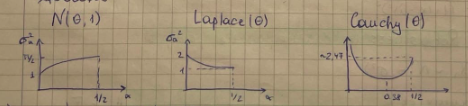
\includegraphics[width=\linewidth]{graphs_are.png}
    \caption{Ас. эффективность усечённых средних}
\end{figure}
\begin{namedtheorem}
    Пусть $\disp_\theta X_1 < + \infty$, тогда
    $$
        ARE_{\overline{X_\alpha}, \overline{X}} \leq (1-2\alpha)^2 
    $$
\end{namedtheorem}
Доказательство:
$$
    \frac{1}{2}\disp_\theta X_1 = \frac{1}{2}\int_\R x^2p_\theta(x) dx  = \int_{0}^{\infty} x^2p_\theta(x)dx = 
    \left(\int_{0}^{u_{1-\alpha}} dx + \int^{u_{1-\alpha}^\infty} dx\right)x^2p_\theta(x) \geq 
    $$
    $$
    \geq u_{1-\alpha}^2\alpha
    + \int_{0}^{u_{1-\alpha}}x^2p_\theta(x) dx = \frac{(1-2\alpha^2)}{2}\sigma_\alpha^2
$$
\subsubsection{Медиана средних Уолша}
\begin{dfn}
    Обозначим $Y_{i, j} = \frac{X_i + X_j}{2}, 1 \leq i \leq j \leq n$  - средние Уолша. Тогда медианой средних 
    Уолша называется число $W$ - медиана всех $Y_{i, j}$
\end{dfn}
\begin{namedtheorem}
    Пусть $\sample \sim P_\theta \in \mathcal{P}$, тогда медиана средних Уолша - а.н.о. для $\theta$, причём ас. дисперсия 
    выражается как:
    $$
        \sigma^2 = \frac{1}{12\left(\int_\R p_\theta^2(x) dx\right)^2}
    $$
\end{namedtheorem}
\begin{annotation}
    Для $P_\theta \in \mathcal{P} \quad ARE_{W, \overline{X}} \geq \frac{108}{125}\approx 0.864$ \\ 
    $\tau_W \approx 0.293 \Rightarrow W$ устойчива к 29\% выбросов 
\end{annotation}


\section{Проверка статистических гипотез}
\subsection{Гипотезы и критерии}
Пусть $\mathcal{X}$ - выборочное пространство, $\mathcal{P}$ - семейство распределений на нём. Рассматриваются высказывания вида:
\begin{itemize}
    \item $H_0: \quad P \in P_0$ - основная гипотеза
    \item $H_1: \quad P \in P_1$ - альтернативная гипотеза 
\end{itemize}
Где $P_0, P_1 \in \mathcal{P}, \,\, P_0\bigcap P_1 = \emptyset$. Для параметрического подхода гипотезы имеют вид:
\begin{itemize}
    \item $H_0: \quad \theta \in \Theta_0$
    \item $H_0: \quad \theta \in \Theta_1$
\end{itemize}
Где $\Theta_0, \Theta_1 \subseteq \Theta, \quad \Theta_0 \bigcap \Theta_1 = \emptyset$
\begin{annotation}
    Не обязательно, чтобы $\Theta_0 \bigcup \Theta_1 = \Theta$. Например, гипотезы могут быть:
    \begin{enumerate}
        \item $H_0: \theta = \theta_0 \quad vs. \quad H_1: \theta > \theta_0$ - правосторонняя альтернатива
        \item $H_0: \theta = \theta_0 \quad vs. \quad H_1: \theta < \theta_0$ - левостороннаяя альтернатива
        \item $H_0: \theta = \theta_0 \quad vs. \quad H_1: \theta \neq \theta_0$ - двусторонняя альтернатива
    \end{enumerate}
    Истинное $\theta$ может не удовлетворять ни одной. 
\end{annotation} 
Примеры:
\begin{enumerate}
    \item $\mathcal{P} = \{$все абс. непр. распределения$\}$\\ $H_0: \,\, P \sim \normal{a}{\sigma^2}$, 
    $H_1: \,\, P \sim \exp(\lambda)$
    \item $\mathcal{P} = \{ \normal{a}{\sigma^2}: a \in \R, \sigma > 0\}$\\ $H_0: \,\, a = 0$, $H_1: a > 0$
\end{enumerate}
\begin{dfn}
    Подмножество $S\subseteq \mathcal{X}$ называется критерием проверки $H_0 vs. H_1$, если правило отвержения 
    гипотезы $H_0$ при выборке $X$ имеет вид:
    $$
        H_0 \text{отвергается} \Leftrightarrow X \in S
    $$
\end{dfn}
Часто используется следующий частный случай: Берут некоторую статистику $T(X)$, а в качестве критерия выбирают множество:
$$
    S = \{ X | T(x) > c \}
$$
Для некоторого $c$, которое называется в данном случае критическим значением. Правило отвержения в этом случае будет записываться как:
$$
H_0 \text{отвергается} \Leftrightarrow T(X) > c
$$
\begin{dfn}
    Пусть $S$ - критерий для проверки $H_0 vs. H_1$. Тогда:
    \begin{itemize}
        \item $X \in S \Rightarrow H_0$ - отвергается, то результат тестирования \textbf{статистически значим}
        \item \item $X \not\in S \Rightarrow H_0$ - не отвергается, то результат тестирования \textbf{статистически незначим}
    \end{itemize}
\end{dfn}
\begin{annotation}
    В общем случае неверно, что если $H_0$ отвергается, то принимается $H_1$. Этот приницип схож с приниципом презумпции невиновности: \\
    \textbf{Каждый обвиняемый в совершении преступления считается невиновным, пока его виновность не будет доказана в предусмотренном законом порядке и установлена вступившим в законную силу приговором суда}
    Аналогию с судом можно продолжить:
    \begin{center}
    \begin{tabular}{ |c| c| c| }
        \hline
         Обвиняемый & $P$ - неизвестное распределение \\ 
         \hline
         Невиновность & $H_0 : P \in P_0$  \\  
        \hline         
         Виновность & $H_1: P \in P_1$ \\
         \hline    
         Преступление & $X = (X_1, ..., X_n)$ - выборка \\
         \hline
         Улики и доказательства & $T(X)$ - статистика критерия \\
         \hline 
         Доказательство виновности & Справедливость $X\in S$ \\
         \hline
    \end{tabular}
    \end{center}
\end{annotation}
При проверке гипотез могут возникать ошибки. Ошибки бывают двух сортов: первого и второго. 
\begin{center}
    \begin{tabular}{ |c| c| c| }
         \hline    
          & $H_0$ верна & $H_0$  неверна  \\
         \hline
         $H_0$ не отв. & =) &  II \\
         \hline 
         $H_0$ отв. & I  & =) \\
         \hline
    \end{tabular}
    \end{center}
\begin{dfn}
Ошибка первого рода - ситуация, в которой мы отвергли верную гипотезу. Ошибка второго рода - 
ситуация, в которой мы не отвергли ложную гипотезу.
\end{dfn}
\begin{dfn}
    Вероятности ошибки (хотя это совсем не вероятность), принято называть следующие величины:
    \begin{enumerate}
        \item Вероятность ошибки первого рода: $P(I_S) = \sup\limits_{P\in P_0} P(X\in S)$
        \item Вероятность ошибки второго рода: $P(II_S) = \sup\limits_{P\in P_1} P(X\not \in S)$
    \end{enumerate}
    \end{dfn}    
Ошибки первого рода считаются более опасными. Поэтому обычно решается задача:
\begin{equation}
    \begin{split}
        P(I_S) &\leq \alpha \\    
        P(I\!I_S) &\to \min_S
    \end{split}
\end{equation}
\begin{dfn}
    Уровнем значимости критерия $S$ называется такое число $\alpha$, что  $P(I_S) \leq \alpha$
    При этом число $\alpha_P = P(I_S)$ называется точным уровнем значимости. 
\end{dfn}
Обычно выбирают $\alpha = 0.05$ - первая магическая константа.  \\
Обычно альтернативы имеют сложный вид:
\begin{itemize}
    \item $H_0: \theta = \theta_0 vs H_1: \theta > \theta_0$
    \item $H_0: P \sim \normal{a}{\sigma^2}  vs H_1: P \not\sim \normal{a}{\sigma^2}$
\end{itemize}
Значит, имеет смысл сравнивать критерии на разных распределениях из альтернативы. Для этого введём:
\begin{dfn}
    $\beta_S(P) = P(X\in S)$ для $P \in \mathcal{P}_1$ - функция мощности. 
\end{dfn}
Пример: Пусть $X$ - выборка из 1 элемента из распределения $Exp(\theta)$. Построить критерий 
уровня значимости $\alpha$ для проверки гипотез $H_0: \theta = \theta_0 vs H_1: \theta > \theta_0$. Заметим, что 
$\expec_\theta X = \frac{1}{\theta} \Rightarrow$ чем больше $\theta$, тем меньше $X$ в среднем. Разумно брать 
критерии вида $S = \{ X < c \}$ где $c$ мы подберём из условия $P(I_S) \leq \alpha$. Выпишем это условие:
$$
    P(I_S) = P_\theta(X < c) = 1 - e^{-\theta_0 c} \leq \alpha \Rightarrow c\leq -\frac{1}{\theta_0}\ln(1-\alpha)
$$
Опеределим мощность полученного критерия:
$$
    \beta_S(\theta) = 1 - \exp(\frac{\theta}{\theta_0}\ln(1-\alpha)) = 1 - (1 - \alpha)^{\frac{\theta}{\theta_0}}
$$
Таким образом, полученный критерий:
$$
    S = \{ X < -\frac{1}{\theta_0}\ln(1-\alpha)\}
$$
Пример с числами: Пусть $\theta_0 = 1, a =0.05 \Rightarrow c = 0.051$. Соответственно, если $X < 0.051$, то 
гпиотеза $H_0$ отвергается (результат стат. значим). Иначе - статистически незначим 
\subsection{Критерий Вальда}
\begin{dfn}
    Критерий $S$ - асимптотический критерий уровня значимости $\alpha$, если 
    $$
    \overline{\lim_{n\to\infty}} P(I_S) \leq \alpha
    $$
\end{dfn}
Пусть $X = (X_1, ..., X_n)$ - выборка из неизвестного распределения $P\in\mathcal{P}, \mathcal{P}= \{P_\theta: \theta \in \Theta 
\subseteq \R^d \}$. Раассмотрим гипотезы:
\begin{enumerate}
    \item $H_0: \theta = \theta_0$
    \item $H_1: \theta = \theta_1$
\end{enumerate}
Пусть у нас есть $\hat\theta$ - ассимптотически нормальная оценка $\theta_0$ с ассимптотической дисперсией $\sigma(\theta_0)^2$, 
а также $\hat\sigma $ - состоятельная оценка $\sigma$. Тогда из свойств а.н.о следует, что:
$$
    W(X) = \sqrt{n}\frac{\hat\theta - \theta_0}{\hat\sigma} \dconv \normal{0}{1}
$$
Таким образом, мы получаем следующий критерий 
\begin{dfn}
    Критерий $S = \{ \sqrt{n}\frac{|\hat\theta - \theta_0|}{\hat\sigma} > z_{\frac{1-\alpha}{2}}\}$
\end{dfn}
Ясно, что это ассимптотический критерий уровни значимости $\alpha$. Изучим мощность данного критерия:
$$
    \beta_S(\theta) = P_\theta(W > z_{1 - \frac{\alpha}{2}}) + P_\theta(W < z_{\frac{\alpha}{2}}) = 
$$
$$
    = P_\theta(\sqrt{n}\frac{\hat\theta - \theta}{\hat\sigma} > z_{1-\frac{\alpha}{2}} - \sqrt{n}\frac{\theta - \theta_0}{\hat\sigma})
    + P_\theta(\sqrt{n}\frac{\hat\theta - \theta}{\hat\sigma} < z_{\frac{\alpha}{2}} - \sqrt{n}\frac{\theta - \theta_0}{\hat\sigma}) \to
$$
$$
    \to 1 - \Phi(z_{1-\frac{\alpha}{2}} - W(\theta)) + \Phi(z_{\frac{\alpha}{2}} - W(\theta))
$$
Замечания: 
\begin{enumerate}
    \item Кртерий Вальда обощается на случай $H_1: \theta > \theta_0$: 
    $$
    S_r = \{\sqrt{n}\frac{\hat\theta - \theta_0}{\hat\sigma} > z_{1-\alpha} \}
    $$
    (уроень значимости $\alpha$ )
    \item Кртерий Вальда обощается на случай $H_1: \theta < \theta_0$: 
    $$
    S_l = \{\sqrt{n}\frac{\hat\theta - \theta_0}{\hat\sigma} < z_{\alpha} \}
    $$
    (уроень значимости $\alpha$ )
    \item Можно рассмотреть доверительный интервал:
    $$
        C = (\hat\theta \pm z_{1-\frac{\alpha}{2}}\frac{\hat\sigma}{\sqrt{n}})
    $$
    Он имеет уровень доверия $1-\alpha$. Тогда $H_0$ отвергается тогда и только тогда, когда
    $\theta_0 \not\in C$.
    \item 
\end{enumerate}
\subsection{Критерии отношения правдоподобия}
Пусть $X =(\sample)$ - выборка из распределения $P\in \mathcal{P}$, где $\mathcal{P} = \{P_\theta, \theta \in \Theta\}$ - 
доминирующее семейство. Попробуем в частных случаях решить задачу:
\begin{equation}
    \begin{cases}
      P(I_S) \leq \alpha\\
      P(I\!I_S) \to \min 
    \end{cases}\
\end{equation}
\begin{enumerate}
    \item Простые гипотезы. \\ 
    Рассмотрим случай: $H_0: \theta = \theta_0 vs. H_1: \theta = \theta_1$. Рассмотрим статистику:
    $$
    \Lambda(X) = \frac{L_X(\theta_1)}{L_X(\theta_0)}
    $$
\begin{namedtheorem}[Лемма Неймана-Пирсона]
    Если $\exists c_\alpha: \quad P_{\theta_0}(\Lambda(X) > c_\alpha) = \alpha$, то критерий 
    $$
        S(X) = \{ \Lambda(X)  > c_\alpha\}
    $$
    является критерием уровня значимости $\alpha$ и наибольшей мощностью из всех таких критериев.
\end{namedtheorem}
    \item Сложные гипотезы \\
    \begin{dfn}
        Критерий $S$ уровня значимости $\alpha$ называется равномерно наиболее мощным критерием (РНМК), если для любого 
        другого критерия $T$ того же уровня значимости выполнено неравенство:
        $$
            \forall P \in P_1: \quad \beta_S(P) \geq \beta_T(P)
        $$
    \end{dfn}
    \begin{namedtheorem}[О монотонном отношении правдоподобия]
        Пусть $\forall \theta_1 > \theta_2$ отношение правдоподобия представимо в виде:
        $$
            \frac{L_X(\theta_1)}{L_X(\theta_2)} = f_{\theta_1, \theta_2}(T(X))
        $$
        Где $T(X)$ - некоторая статистика, а $f_{\theta_1, \theta_2}$ - монотонно возрастающая функция. Тогда критерий:
        $$
            S = \{ T(X)> c_\alpha\}
        $$
        является РНМК с уровнем значимости $\alpha$ для проверки гипотез 
        $$
            H_0: \theta = \theta_0\,\, \textrm{vs} \,\,H_1: \theta > \theta_0
        $$
        Где $c_\alpha$ подбирается из условия $P_{\theta_0}(T(X) > c_\alpha) = \alpha$
    \end{namedtheorem}
\end{enumerate} 
Пример: Рассмотрим $(\sample) \sim Exp(\theta)$. Рассмотрим также гипотезы $H_0: \theta = \theta_0, H_1: \theta > \theta_0$.
Требуется найти РМНК. Пусть $\theta_1 > \theta_2$, выпишем отношение правдоподобия:
$$
    \Lambda(X) = \frac{L_X(\theta_1)}{L_X(\theta_2)} = \frac{\theta_1^n \exp(-\theta_1 \sumin X_i)}{\theta_2^n \exp(-\theta_2 \sumin X_i)} =
    \left(\frac{\theta_1}{\theta_2}\right)^n \exp\left[-(\theta_1 - \theta_2)\left(\sumin X_i\right)\right]
$$
Тогда для статистики $T(X) = \sumin X_i$ выполняются условия теормы о монотонном отношении правдоподобия. Полученный критерий:
$$
    S = \{T(X) < c_\alpha \}
$$
Где $c_\alpha$ находится из условия $P_{\theta_0}(T(X) < c_\alpha) = \alpha$. Мы знаем из курса ТВ, что $T(X) \sim \Gamma(\theta_0, n)$. 
В таком случае, $c_\alpha$ - $\alpha$ квантиль распределения $\Gamma(\theta_0, n)$

\section{Непараметрический подход}
\subsection{Эмперическое распределение}
Пусть $X=(\sample)$ - выборка из распределения $P \in \mathcal{P}$. 
\begin{dfn}
    Распределение $\hat P_n(X)$ - эмперическое распределение по выборке $X$, если для любого множества $B \in \mathcal{B}$:
    $$
        \hat P_n(B) = \frac{1}{n}\sumin I \{ X_i \in B\}
    $$
\end{dfn}
Заметим следующие свойства:
\begin{enumerate}
    \item $\hat P_n(B)$ - случайная величина, доля элементов, попавших в $B$.
    \item $\hat P_n$ - случайная вероятностная мера. 
    \item $n \hat P_n (B) \sim B(n, P(B))$
    \item $\expec \hat P_n(B) = P(B)$
    \item $\disp \hat P_n(B) = \frac{p(1-p)}{n}$/
    \item $\hat P_n(B) \sconv P(B)$
\end{enumerate}
Рассмотрим случай $(\R, \mathcal{B(\R)})$. Тогда $\hat P_n$ соответствует эмпирической функции распределения. Можно 
определить эмперичческую функцию распределения
\begin{dfn}
    Эмпирической функцией распределения называется функция:
    $$
        \hat F_n(x) = \hat P_n(x) = \frac{1}{n}\sumin I\{ X_i \leq x\}
    $$
\end{dfn}
Тогда истинно утверждение: $\hat F_n(x) \sconv F(x)$. Более того, верна следующая
\begin{namedtheorem}[Гливенко-Кантелли]
    Если $F$ - функция распределения для $P, (\sample) \sim P$, тогда верно: 
    $$
        D_n = \sup_{x\in R} |\hat F_n(x) - F(x)| \sconv 0
    $$
\end{namedtheorem}
Заметим также, что $D_n = \sup_{B \in \mathcal{A}} | \hat P_n(B) - P(B)|$, 
$\mathcal{A} = \{(-\infty, x], x \in \R\}$. Эту теорему можно обобщить 
и на другие $\mathcal{A}$. Например: $\mathcal{A} = \{ \text{Все объединения интервалов в количестве 
не более $k$ штук}\}$. На любые конечные объединения обобщить нельзя. 
\begin{namedtheorem}[Вапника-Червоненкинса]
    $$
        \sup_{B\in \mathcal{A}} |\hat P_n(B) - P(B)| \sconv 0 \Leftrightarrow dim_{VC} < \infty 
    $$      
    При разбиении $\R^d$ множествами из $\mathcal{A}$
\end{namedtheorem}
\begin{namedtheorem}[Колмогорова-Смирнова]
    Рассмотрим $\sqrt{n}D_n$. Утверждается, что 
    $$
        \sqrt{n}D_n \dconvt \xi
    $$
    Где $\xi \sim Kolmogorov$  - распределение Колмогорова, его функция распределения:
    $$
        F_\xi(x) = \sum{k=-\infty}^\infty (-1)^ke^{-2k^2x^2}I\{x \geq 0\}
    $$
\end{namedtheorem}
\begin{annotation}
    Скорость сходимости: $\sqrt{N}$
\end{annotation}
\subsection{Метод подстановки}
\begin{dfn}
    Пусть $X = (\sample) \in P, F$ - функция распределения. Пусть также $\theta = G(P)$ - 
    параметр, значение которого хотим оценить. Тогда оценкой по методу подстановки называют 
    $\hat\theta = G(\hat p_n)$ - оценка методом подстановки    
\end{dfn}
Примеры:
\begin{enumerate}
    \item $\theta = G(P) = \expec_P f(X_1) = \int_\R f(x) dF(x)$ - линейный функционал. Тогда $\hat\theta = \expec_{\hat p_n} f(x_1) 
    = \overline{f(x_i)}$
    \item $G(P) = \disp_P (x_1) = \expec_P(x_1^2) - \expec_p(x_1)^2$.Тогда получаем 
    $$
        \hat \theta = \overline{X^2} - \overline{X}^2 = S^2
    $$
    \item $\theta = G(P) = F^{-1}(\alpha) = \min \{x | \hat F_n(x) \geq \alpha \} = \orst{X}{\lceil n\alpha \rceil}$
\end{enumerate}

\end{document} % Конец текста.x

